\documentclass[11pt]{article}
\usepackage[margin=1.05in]{geometry}
\usepackage{amsmath,amssymb,booktabs}
\usepackage{graphicx}
\usepackage[expansion=false]{microtype}
\usepackage[font=small,labelfont=bf,skip=5pt]{caption}
\usepackage[colorlinks=true,linkcolor=black,citecolor=black,urlcolor=blue]{hyperref}
\usepackage{titlesec}
\titlespacing{\section}{0pt}{1.35em}{0.5em}
\titlespacing{\subsection}{0pt}{1.0em}{0.35em}
\setlength{\parskip}{0.35em}
\renewcommand{\topfraction}{0.92}
\renewcommand{\bottomfraction}{0.75}
\renewcommand{\textfraction}{0.06}
\renewcommand{\floatpagefraction}{0.85}
\newcommand{\rs}{$r^{*}$}

\begin{document}

\begin{center}
{\large\textbf{The FOMC Window}}\\[0.3em]
{\normalsize What is identified, what is not, and where the project goes next}\\[0.5em]
{\small Progress report \textperiodcentered\ 11 August 2026}
\end{center}
\vspace{0.3em}
\noindent\rule{\textwidth}{0.4pt}
\suppressfloats[t]

% =====================================================================
\section{The motivating fact}

The starting point is Hillenbrand (2025, \emph{RFS}). Between June 1989 and June 2021 the
ten-year Treasury yield fell 6.99 percentage points. Of that, 6.16 pp --- 88\% --- accrued
inside three-day windows around FOMC announcements (days $t-1$, $t$, $t+1$), which are only
11.8\% of trading days. On the other 88\% of days the yield went essentially nowhere.

I replicate the result from Gürkaynak--Sack--Wright zero-coupon yields and a
hand-assembled FOMC calendar (300 scheduled meetings 1989--2026 plus 73 conference calls
and unscheduled actions). Figure~\ref{fig:fact} reproduces it.

\begin{figure}[tbp]
\centering
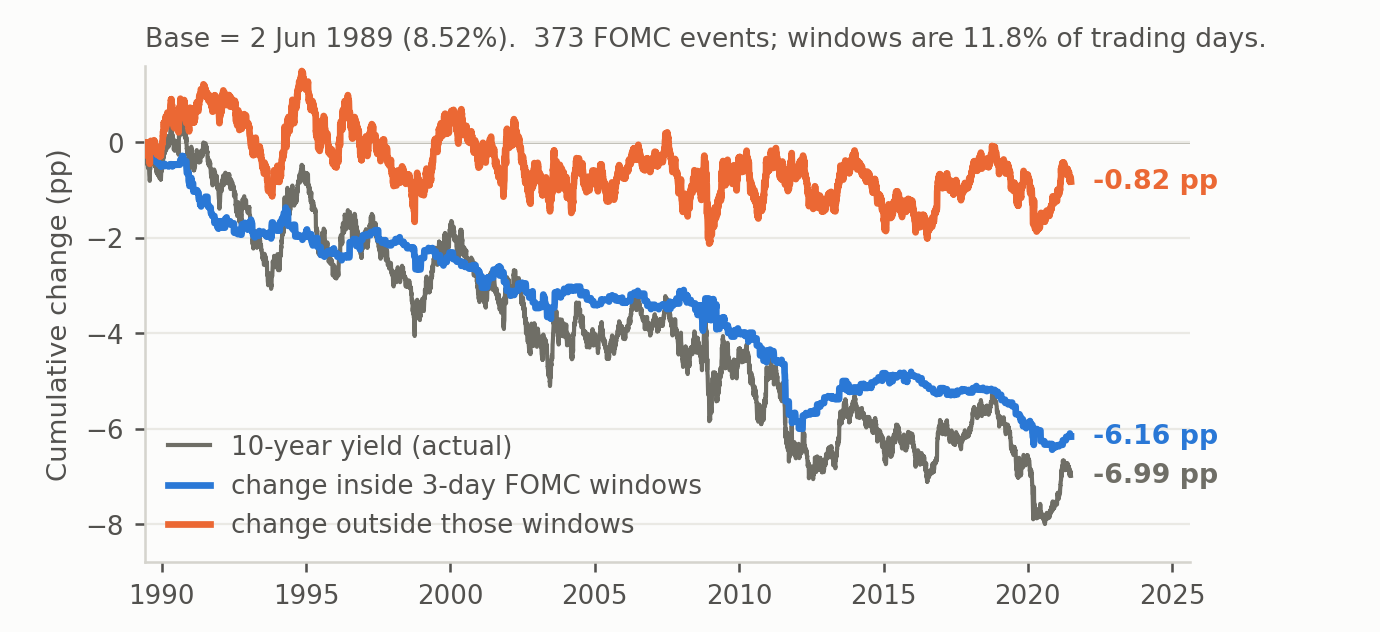
\includegraphics[width=0.95\textwidth]{s_fact.png}
\caption{\textbf{Long rates fall only when the Fed is in the room.} Cumulative change in the
ten-year yield from 2 June 1989 (8.52\%), split into the part accruing inside three-day FOMC
windows and the part accruing on all other days. Paper sample, through June 2021.}
\label{fig:fact}
\end{figure}

\subsection{The fact is really an absence}

It is worth being precise about what is surprising here, because the per-meeting effect is
small: about $-2.5$ bp. The striking quantity is the \emph{non}-window drift, which is
$-0.012$ bp/day with $t=-0.18$ across 7{,}035 days. Thirty-two years of macroeconomic news,
inflation surprises, recessions and QE announcements net out to zero outside a
three-day calendar.

A randomisation test confirms the concentration is not chance: placing 324 randomly timed
three-day blocks on non-FOMC days, 5{,}000 times, puts the observed $-6.16$ pp at the 0th
percentile of the simulated distribution ($p<0.0002$).

The two day types are not distinguished by volatility. Window days have a daily standard
deviation of 6.72 bp against 5.60 bp elsewhere --- a 20\% difference. They are distinguished
by \emph{drift}: $-0.634$ bp/day against $-0.012$. The drift-to-noise ratio is roughly
45 times higher inside the window (Figure~\ref{fig:persist}). Announcement days are not
noisier days; they are days on which the noise does not cancel.

\begin{figure}[tbp]
\centering
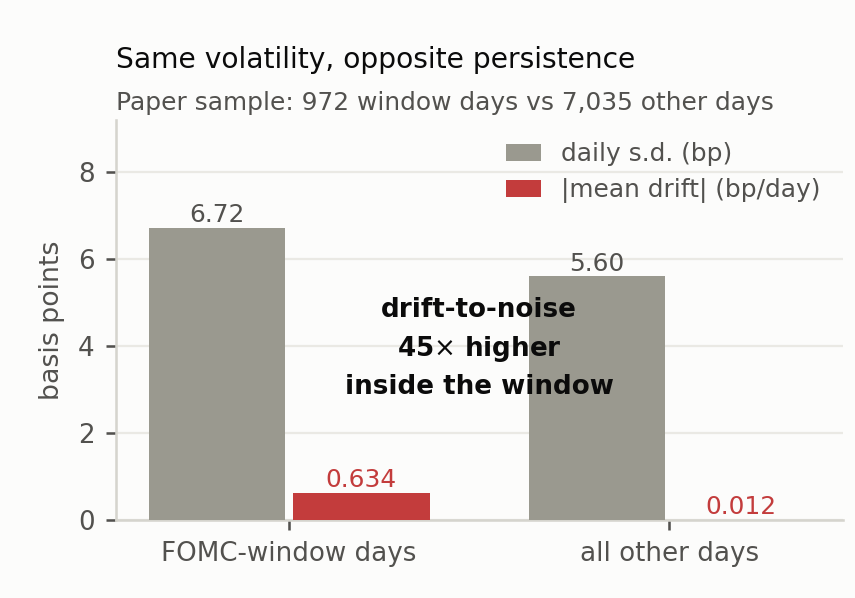
\includegraphics[width=0.62\textwidth]{s_persist.png}
\caption{\textbf{Same volatility, opposite persistence.} Daily standard deviation and absolute
mean drift of ten-year yield changes, window days versus all other days, June 1989 -- June 2021.}
\label{fig:persist}
\end{figure}

\subsection{Hillenbrand's explanation: long-run Fed guidance}

Hillenbrand's own interpretation is that FOMC announcements are the moments at which the Fed
reveals information about \emph{where rates are going in the long run} --- what he calls
\textbf{long-run Fed guidance}. The premise is an information asymmetry: by continuously
observing how the economy responds to the rates it sets, the Fed accumulates an estimate of
the natural rate that markets cannot form as precisely on their own. Investors learn that
estimate at announcements and reprice long-duration bonds accordingly. Because the object
being revised is an \emph{endpoint} rather than a cyclical position, the revision is
permanent, and permanent revisions cumulate rather than cancel --- which is exactly the
pattern in Figure~\ref{fig:fact}.

He describes the guidance as operating through two channels:

\begin{itemize}\setlength\itemsep{0.15em}
\item \textbf{Implicit, before 2012.} When the Fed moves the funds rate, the move itself
reveals its reading of where the natural rate sits. Consistent with this, the meetings at
which the target changed --- roughly 45\% of meetings in his pre-2012 sample --- account for
almost the entire decline in long yields over that period.
\item \textbf{Explicit, from 2012.} The SEP dot plot publishes each participant's longer-run
federal funds projection, communicating the Fed's endpoint view directly.
\end{itemize}

\noindent Four pieces of evidence are offered that the object being moved is a long-run
\emph{real} endpoint rather than the cycle, inflation, or a risk premium.

\begin{enumerate}\setlength\itemsep{0.2em}
\item \textbf{Far-forward rates.} The pattern holds for the 5-year, 5-year-forward rate, where
the current policy stance has largely washed out. A cyclical explanation should not survive
that far out the curve.
\item \textbf{Real rather than inflation.} Since 1999 the decline is essentially all in TIPS
yields, with breakeven inflation roughly flat --- so it is $\Delta r^{*}$, not $\Delta\pi^{*}$.
\item \textbf{The dot plot links the two legs directly.} Regressing window changes in
long-term real yields on revisions to the Fed's longer-run projection, a 100 bp cut in the
Fed's own long-run forecast is associated with more than a 70 bp fall in long-term real
yields --- a pass-through large enough to be about the endpoint rather than the near path.
\item \textbf{Persistence.} The series built only from window changes tracks the low-frequency
movement of the ten-year closely, while the non-window series is transitory and offsets over
time. Endpoint news should not reverse; cyclical or liquidity-driven news should.
\end{enumerate}

\noindent In terms of the identity developed in \S\ref{sec:identity}, the claim is a strong
one: in FOMC windows $\Delta y^{(n)} \approx \Delta r^{*}$, with the inflation anchor, the
policy-stance terms and the term premium all contributing approximately nothing. Each of
those three exclusions is a separate assumption, and the rest of this report is largely about
which of them survive.

% =====================================================================
\section{The question}

If the Fed sets an overnight rate, why does the \emph{ten-year} rate move only on its
calendar --- and why do those moves not wash out? The question I set out to answer is which
component of the yield the Fed is moving:

\begin{quote}
When the Fed moves long rates at scheduled announcements, is it changing \textbf{where markets
think rates are going} (expected future short rates), or \textbf{what markets charge for the risk
of being wrong about that} (the term premium)?
\end{quote}

\subsection{Unpacking the identity}
\label{sec:identity}

The reason this leads directly to \rs{} is an accounting identity, and it is worth writing
out in full because the interesting term is the one usually waved away.

Start from the definition of a long yield as an average of expected short rates plus a
residual:
\begin{equation}
y^{(n)}_t \;=\; \underbrace{\frac{1}{n}\sum_{j=0}^{n-1} E_t\!\left[i_{t+j}\right]}_{\text{expectations component } rn^{(n)}_t} \;+\; TP^{(n)}_t .
\label{eq:eh}
\end{equation}
This is a definition, not an assumption: $TP^{(n)}_t$ is whatever is left over.

Now split the nominal policy rate into a neutral level and a deviation from it. Define the
\emph{neutral nominal rate} and the \emph{policy gap}
\begin{equation}
i^{*}_t \;\equiv\; r^{*}_t + \pi^{*}_t ,
\qquad
\text{gap}_t \;\equiv\; i_t - i^{*}_t \;=\; \underbrace{\left(i_t - E_t\pi_{t+1} - r^{*}_t\right)}_{\text{real policy stance}} \;+\; \underbrace{\left(E_t\pi_{t+1} - \pi^{*}_t\right)}_{\text{inflation deviation}} ,
\label{eq:gapdef}
\end{equation}
where $r^{*}_t$ is the equilibrium real rate and $\pi^{*}_t$ the long-run inflation
anchor. The gap is therefore \textbf{the stance of policy}: how far the Fed is holding the
short rate above or below the level that would be neutral, plus how far inflation is
expected to run from its anchor. Under a Taylor-type rule
$i_t = i^{*}_t + \phi_\pi(\pi_t-\pi^{*}_t) + \phi_x x_t + v_t$, the gap is exactly the
systematic and discretionary response to the cycle,
\begin{equation}
\text{gap}_t \;=\; \phi_\pi\!\left(\pi_t-\pi^{*}_t\right) + \phi_x x_t + v_t .
\label{eq:taylor}
\end{equation}
It is a cyclical, mean-reverting object: it is large in 1994, in 2008 and in 2023, and zero
on average.

Substituting \eqref{eq:gapdef} into \eqref{eq:eh} and adding the assumption that the
endpoints are (locally) martingales, $E_t[r^{*}_{t+j}]=r^{*}_t$ and
$E_t[\pi^{*}_{t+j}]=\pi^{*}_t$, gives the identity used throughout:
\begin{equation}
y^{(n)}_t \;=\; r^{*}_t \;+\; \pi^{*}_t \;+\; \frac{1}{n}\sum_{j=0}^{n-1} E_t\!\left[\text{gap}_{t+j}\right] \;+\; TP^{(n)}_t .
\label{eq:identity}
\end{equation}

\subsubsection*{How much does the gap term actually contribute?}

The usual move at this point is to say the gap ``averages out'' at a ten-year horizon. That
is too quick, and it is the step I initially got wrong. If the gap mean-reverts as an AR(1)
with monthly persistence $\rho$, then
\begin{equation}
\frac{1}{n}\sum_{j=0}^{n-1} E_t\!\left[\text{gap}_{t+j}\right]
\;=\; \omega(\rho,n)\,\text{gap}_t ,
\qquad
\omega(\rho,n) \;=\; \frac{1-\rho^{\,n}}{n\,(1-\rho)} .
\label{eq:omega}
\end{equation}
The weight $\omega$ is small but not zero:

\begin{center}\small
\begin{tabular}{lccc}
\toprule
Half-life of the gap & $\omega$, 2-year & $\omega$, 5-year & $\omega$, 10-year\\ \midrule
1 year  & 0.56 & 0.29 & 0.15\\
2 years & 0.73 & 0.48 & 0.28\\
3 years & 0.81 & 0.60 & 0.39\\
4 years & 0.85 & 0.67 & 0.48\\
\bottomrule\end{tabular}
\end{center}

\noindent So a 100 bp change in the perceived policy stance --- with no change whatsoever in
\rs{}, $\pi^{*}$ or the term premium --- moves the ten-year by 15 to 48 bp, depending on how
persistent markets think the stance is. Differencing \eqref{eq:identity} over an
announcement window,
\begin{equation}
\Delta y^{(n)}_t \;=\; \underbrace{\Delta r^{*}_t + \Delta \pi^{*}_t}_{\text{endpoint news}}
\;+\; \underbrace{\omega\,\Delta\text{gap}_t + \text{gap}_t\,\Delta\omega}_{\text{stance and persistence news}}
\;+\; \Delta TP^{(n)}_t ,
\label{eq:windowdiff}
\end{equation}
which makes the identification problem explicit. Four terms, one observable.

\subsubsection*{Three consequences for the project}

\textbf{1. ``The Fed moves long rates'' does not imply ``the Fed moves \rs{} beliefs.''} The
second term in \eqref{eq:windowdiff} is a live alternative: a meeting that changes how long
markets expect the current stance to last moves the ten-year without touching any endpoint.
The $\text{gap}_t\,\Delta\omega$ piece is particularly awkward, because it is largest exactly
when the stance is large --- 2008--09 and 2022--24 --- and it is what Bauer, Pflueger \&
Sunderam's perceived-reaction-function result is picking up.

\textbf{2. $\pi^{*}$ is not fixed over most of the sample.} The claim that the inflation
anchor is constant is defensible after roughly 2000 and indefensible before it: the 1989--1999
window declines coincide with the disinflation and with the Fed acquiring credibility, so
$\Delta\pi^{*}$ plausibly carries a large share of them. Since 81\% of the in-window decline
predates 2012 (\S5.3), this is not a small caveat --- it means the pre-2012 evidence cannot
be read as \rs{} learning either. TIPS breakevens begin in 1997 (liquid from about 2003), so
the decomposition is only testable on the back half.

\textbf{3. The identity is what makes the term-premium question sharp.} If $\Delta\pi^{*}$ and
the stance terms could be shut down, then a permanent window move in the ten-year would have
to be $\Delta r^{*}$ or $\Delta TP$, and the whole question reduces to splitting those two.
That is the design in \S5 --- and it is why the failure of the market-side endpoint measure
is fatal rather than inconvenient.

% =====================================================================
\section{What the literature has established}

\subsection{The core fact and its extensions}

\noindent
\begin{tabular}{@{}p{0.27\textwidth}p{0.68\textwidth}@{}}
\toprule
\textbf{Paper} & \textbf{What it establishes}\\ \midrule
Hillenbrand (2025, \emph{RFS}) & The whole secular decline in the ten-year accumulates in
three-day FOMC windows, 1989--2021. Attributes it to markets learning a lower \rs{} from
the Fed.\\[0.35em]
Hofmann, Li \& Wu (BIS WP 1252) & The pattern is global --- ten advanced economies --- and
survives a shifting-endpoint model.\\[0.35em]
Hanson, Lucca \& Wright (2021, \emph{QJE}) & Announcement-window long-rate moves
\emph{substantially reverse} within 6--12 months, which they read as evidence of temporary
term-premium effects.\\[0.35em]
Bauer \& Swanson (2023, \emph{NBER Macro Annual}) & Announcement surprises are predictable
from pre-meeting public data; the ``Fed information effect'' is largely the Fed responding
to news.\\
\bottomrule
\end{tabular}

\vspace{0.5em}
\noindent Rows 1 and 3 are in direct tension. Hillenbrand's central fact requires that window
moves \emph{not} reverse --- they have to cumulate into a 32-year trend. Hanson--Lucca--Wright
report that they largely do reverse. The two claims have never been confronted directly.

\subsection{The contested channel}

\noindent
\begin{tabular}{@{}p{0.27\textwidth}p{0.68\textwidth}@{}}
\toprule
\textbf{Paper} & \textbf{What it establishes}\\ \midrule
Hofmann, Li \& Wu (BIS WP 1252) & The window decline is \textbf{risk-neutral} (US pseudo-$R^2$
96 versus 32). But their shifting endpoint is \emph{defined} as the first principal component
of cumulative FOMC-window yield changes, so the risk-neutral component inherits the series
being explained.\\[0.35em]
Pan \& Peng (SSRN 4764451) & On day $t-1$ the decline is \textbf{term premium}: $-0.71$ bp of a
$-0.79$ bp move, with expectations $-0.08$ and insignificant.\\[0.35em]
Joslin, Singleton \& Zhu (2011); Joslin, Priebsch \& Singleton (2014) & Under spanning the
state is recoverable from yields, so the expectations component is a fixed linear function
of the curve.\\[0.35em]
Bauer \& Rudebusch (2020, \emph{AER}); (2014, \emph{IJCB}) & A stationary VAR books genuine
endpoint shifts as term premium: 75\% versus 35--37\% for the secular decline.\\
\bottomrule
\end{tabular}

\vspace{0.5em}
\noindent Two papers, opposite answers, no adjudication. Hillenbrand himself reports in the
Internet Appendix that ACM and Kim--Wright term premia fall 100--200 bp in these windows,
then sets the finding aside because the models ``do not explicitly account for the secular
decline'' --- a reason the measurement is unreliable, not evidence the channel is absent.

\subsection{The beliefs-about-\rs{} strand}

\noindent
\begin{tabular}{@{}p{0.27\textwidth}p{0.68\textwidth}@{}}
\toprule
\textbf{Paper} & \textbf{What it establishes}\\ \midrule
Bauer, Pflueger \& Sunderam (2024, \emph{QJE}) & A pre-meeting \emph{subjective belief} --- the
market's perceived policy reaction-function \emph{slope} --- is related to term premia and to
state-dependent announcement-window responses. This is the template for the design.\\[0.35em]
Ahonon \& Roussellet (FRBNY SR 1187) & Under Bayesian learning about unobserved trends,
investor uncertainty about \rs{} is roughly $\pm$170 bp rather than $\pm$55 bp, and \rs{} is
the primary long-run driver of bond risk premia.\\[0.35em]
Couture (2021); Engstrom (FEDS 2026-026) & The dot plot moves asset prices; SEP-minus-market
gaps predict forecast errors.\\[0.35em]
Favero, Melone \& Tamoni (2024, \emph{JFQA}) & A policy-rate-minus-equilibrium-rate gap predicts
bond returns. Different wedge, similar name --- must be differentiated explicitly.\\
\bottomrule
\end{tabular}

\vspace{0.5em}
\noindent What has never been tested is the perceived \emph{endpoint}: not how strongly markets
think the Fed responds, but where markets think the Fed is heading relative to where the Fed
says it is heading.

% =====================================================================
\section{What our extensions add}

\subsection{Extension 1: the event list decides the answer}

Pan \& Peng and Hofmann--Li--Wu reach opposite conclusions on the same question. I reproduce
Pan \& Peng's estimates on their specification --- scheduled meetings only, September 1994
onward, day $t-1$ --- to three coefficients:

\begin{center}\small
\begin{tabular}{lcc}
\toprule
Day $t-1$, ten-year & Mine & Theirs\\ \midrule
Yield & $-0.785$ ($t\,{-}2.37$) & $-0.79$ ($t\,{-}2.39$)\\
Term premium & $-0.716$ ($t\,{-}2.26$) & $-0.71$ ($t\,{-}2.34$)\\
Expected short rate & $-0.070$ ($t\,{-}0.31$) & $-0.08$ ($t\,{-}0.26$)\\
\bottomrule\end{tabular}
\end{center}

\noindent and then show the attribution is not robust to the event list. Running the same
regression on a $2\times2$ of \{scheduled only, all events\} $\times$ \{1994+, 1989+\} gives:

\begin{center}\small
\begin{tabular}{lrrrrr}
\toprule
Sample & $n$ & Total & Expectations & Term premium & TP share\\ \midrule
Scheduled, 1994+ (P\&P) & 250 & $-0.785$ & $-0.070$ & $-0.716$ & \textbf{91\%}\\
Scheduled, 1989+ & 292 & $-0.755$ & $-0.039$ & $-0.717$ & 95\%\\
All events, 1994+ & 286 & $-0.967$ & $-0.415$ & $-0.552$ & 57\%\\
All events, 1989+ & 364 & $-0.971$ & $-0.521$ & $-0.450$ & \textbf{46\%}\\
\bottomrule\end{tabular}
\end{center}

\noindent bp per event; HAC(4) standard errors; sample ends December 2025.

The event list does the work, not the sample start. Holding the list at ``scheduled,''
moving the start from 1994 to 1989 changes the term-premium share from 91\% to 95\%. Holding
the start at 1994 and adding the unscheduled events changes it from 91\% to 57\%.

The mechanism is identifiable. The 73 conference calls and intermeeting actions that a
scheduled-only filter removes carry $-1.78$ pp of cumulative expectations decline on day
$t-1$ alone --- about $-2.5$ bp per event, against $-0.07$ bp per scheduled meeting, a factor
of 35 (Figure~\ref{fig:eventlist}). Emergency actions are preceded by days of expectations
repricing; scheduled announcements are not.

\begin{figure}[tbp]
\centering
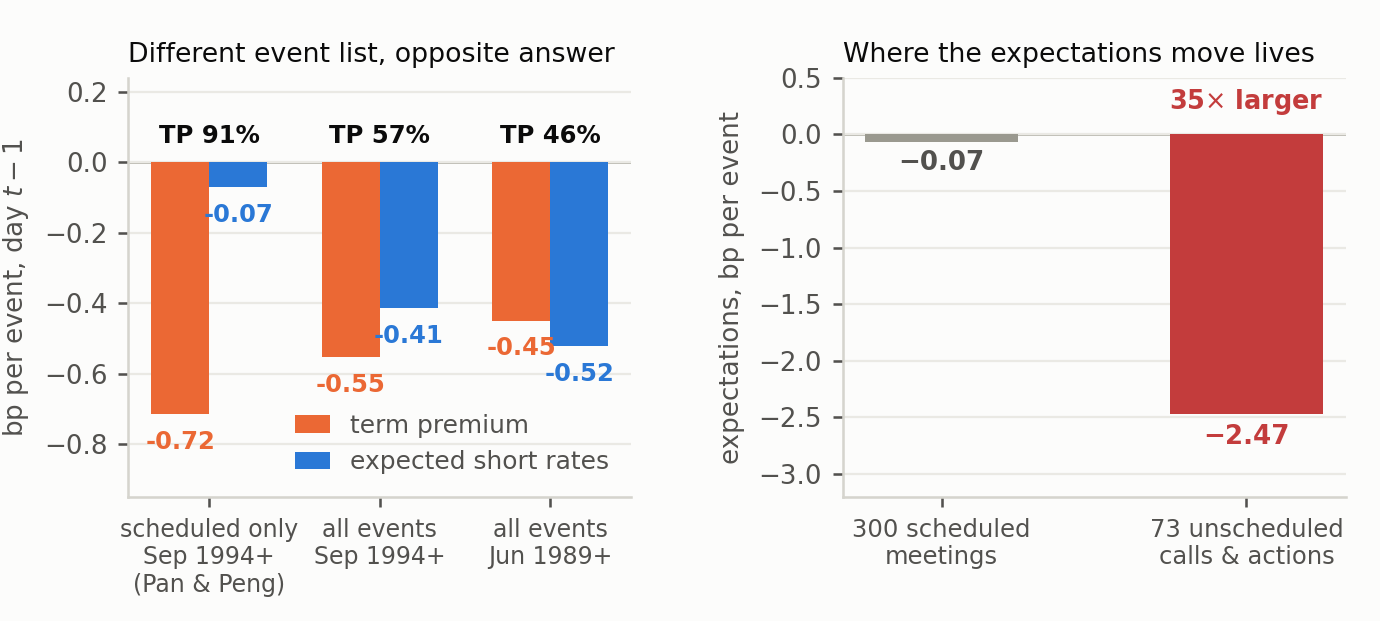
\includegraphics[width=0.95\textwidth]{s_eventlist.png}
\caption{\textbf{The event list decides the answer.} Left: the day-$(t-1)$ decomposition under
three event-list definitions --- same day, same data, same decomposition. Right: the
expectations component per event, scheduled meetings versus unscheduled actions.}
\label{fig:eventlist}
\end{figure}

\emph{What this adds.} The two contradictory papers are reconciled without taking a side on
the model. Neither discusses the event list. This is a finished result requiring no model to
be correct.

\subsection{Extension 2: the sample through July 2026}

Extending the panel to 31 July 2026 covers a period no paper in this literature reaches ---
Hillenbrand ends June 2021, Hofmann--Li--Wu 2023, the Adrian et al.\ vintage November 2021 ---
and it is the one period in the sample in which policy tightened sharply.

Between March 2022 and July 2026 the Fed raised the target range 525 bp and revised its own
longer-run dot \emph{up} by 0.74 pp. The ten-year rose 2.60 pp. Inside FOMC windows it
\emph{fell} 1.20 pp; the entire increase occurred outside (Figure~\ref{fig:extend}). The
in-window series continues its decline straight through the tightening, to $-7.24$ pp.

\begin{figure}[tbp]
\centering
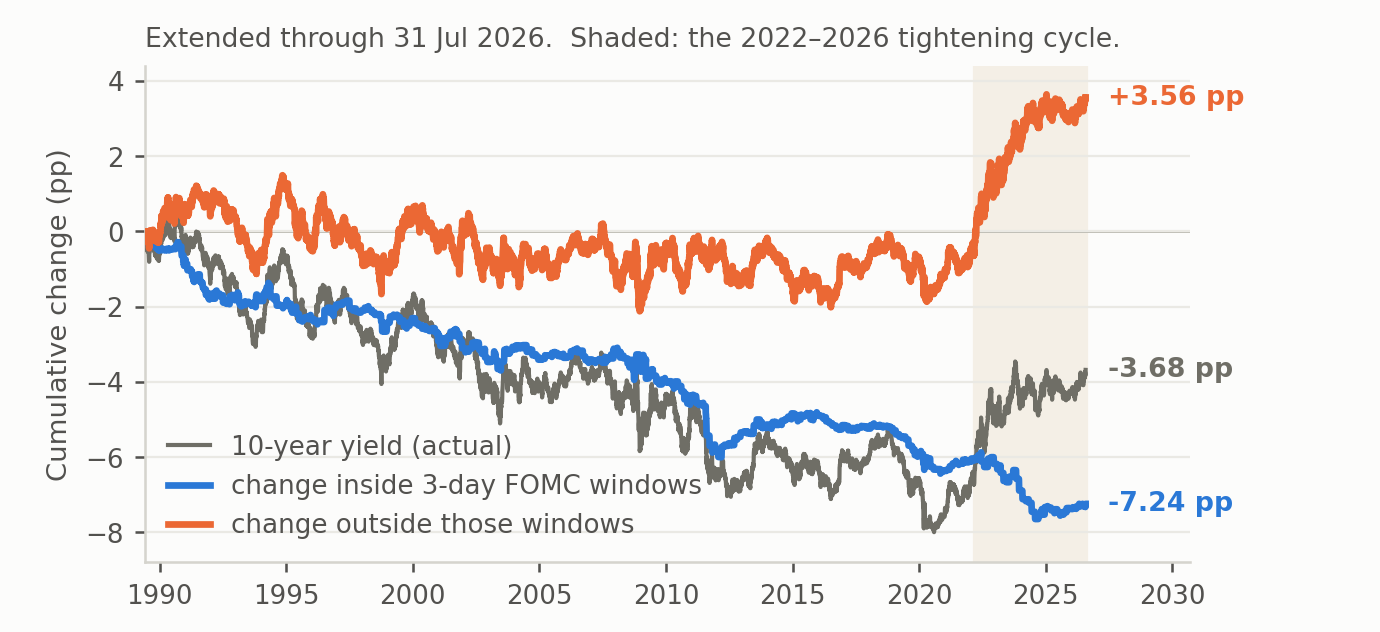
\includegraphics[width=0.95\textwidth]{s_extend.png}
\caption{\textbf{The 2022--2026 tightening happened outside the window.} Same decomposition as
Figure~\ref{fig:fact}, extended to 31 July 2026. Shaded region marks the tightening cycle.}
\label{fig:extend}
\end{figure}

\emph{What this adds.} The pattern is not symmetric in the direction of policy, and the
symmetry assumption is implicit in every existing treatment. It also means the secular-decline
interpretation cannot be the whole story: the in-window decline continued while the Fed was
raising its own \rs{} estimate.

\subsection{Extension 3: the decomposition cannot arbitrate}

Both contested papers rest on an affine decomposition, so it matters what that decomposition
can and cannot deliver at event frequency.

In a spanned affine model the state is recoverable from yields, so the expectations component
is a fixed linear function of the curve:
\begin{equation}
\Delta rn^{(n)}_t \;=\; c_n' \Delta y^{\mathcal N}_t, \qquad c_n' \;=\; b_n' \mathbf{B}^{-1},
\label{eq:filter}
\end{equation}
where $\mathcal N$ is any set of maturities spanning the state. Regressing the daily change in
the ACM ten-year risk-neutral rate on six yield changes (1, 2, 3, 5, 7, 10 years) over
9{,}282 daily observations gives $R^2 = 1.00000$ (Figure~\ref{fig:filter}, left).

The consequence for event studies is immediate: component responses are determined by the
maturity profile of the yield response,
\begin{equation}
\beta^{rn} \;=\; c' \beta^{\mathcal N},
\label{eq:eventcorollary}
\end{equation}
so the decomposition adds \emph{no event-specific information}. Applied to my estimated
profile, \eqref{eq:eventcorollary} predicts $+2.5$ and $+29.3$ bp against directly estimated
$+2.6$ and $+29.2$. Running the decomposition is arithmetic on a profile already in hand.

Those weights are also known to be wrong for this application. Since the VAR is stationary,
$b_n \to 0$ and the expectations component is asymptotically constant, so genuine endpoint
variation is mechanically booked as term premium. Empirically $c'\mathbf{1} = 0.529$: a
permanent, fully credible parallel shift --- 100\% expectations by construction --- is
reported as 53\% expectations and 47\% term premium (Figure~\ref{fig:filter}, right).

\begin{figure}[tbp]
\centering
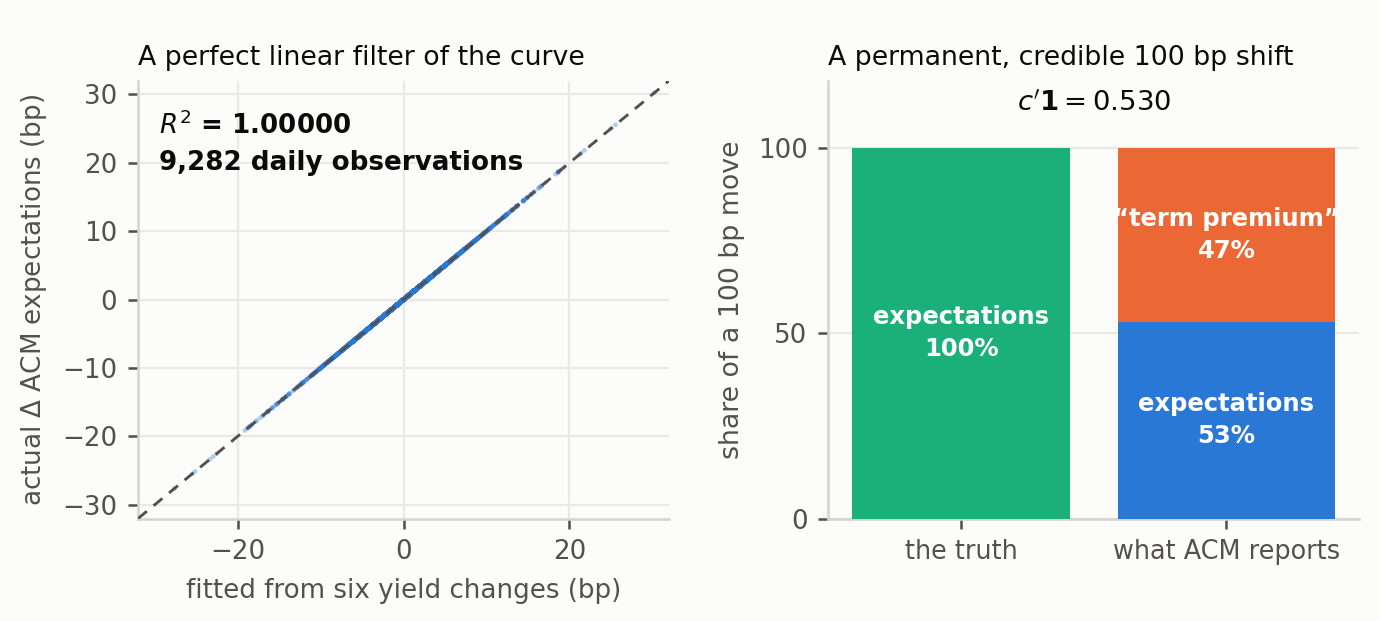
\includegraphics[width=0.95\textwidth]{s_acmfilter.png}
\caption{\textbf{The decomposition is a fixed filter of the curve.} Left: actual daily changes in
the ACM ten-year risk-neutral rate against the fitted values from six contemporaneous yield
changes. Right: how a permanent, fully credible 100 bp parallel shift is reported.}
\label{fig:filter}
\end{figure}

\emph{Attribution.} The algebra in \eqref{eq:filter} is a corollary of Joslin, Singleton \& Zhu
(2011) and appears as a criticism in Joslin, Priebsch \& Singleton (2014). The stationarity
bias is Bauer \& Rudebusch (2020, \emph{AER}), who report 75\% versus 35--37\% for the secular
decline, and Bauer \& Rudebusch (2014), who report the $\approx$50/50 event-window figure. My
contribution is the explicit filter for ACM and the event-study corollary
\eqref{eq:eventcorollary}, not the theorem.

% =====================================================================
\section{Where \rs{} enters}
\label{sec:rstar}

\subsection{The design the identity suggests}

Equation~\eqref{eq:identity} points at a clean test. If the Fed moves long rates by revealing
its own view of the endpoint, then the pre-meeting \emph{gap} between the Fed's published
longer-run projection and the market-implied endpoint should predict the window response ---
and the sign of the loading on the two components should discriminate the mechanisms. An
information channel predicts a signed wedge loading on expectations; a risk channel predicts
the magnitude of disagreement loading on the term premium.

This requires two measured objects: a Fed leg and a market leg.

\subsection{The treatment exists; the control does not}

The Fed leg is real and it moves. The SEP longer-run federal funds projection, less the 2\%
inflation objective, falls 1.78 pp from 2012 to March 2022 and then rises 0.74 pp
(Figure~\ref{fig:rstar}, left). The cross-participant mean has 48 distinct values across 57
meetings, against 12 for the median --- so the mean, not the median, is the usable series.

The market leg fails. The natural candidate --- the ACM 9-year, 1-year-forward risk-neutral
rate --- is not an endpoint estimate at all. Regressed on the change in the one-year yield it
gives $\beta = 0.287$ with $R^2 = 0.83$, and the level correlation is $+0.984$
(Figure~\ref{fig:rstar}, right). It is a damped copy of the current policy cycle.

This is structural rather than a bad horizon choice. Under a stationary VAR the forward
loading $b_n \to 0$, so pushing the horizon out drives the forward toward an unconditional
constant, never toward a time-varying endpoint. No horizon works. Survey-based alternatives
move too little to help: they correlate $-0.12$ with the ACM series and barely vary.

\begin{figure}[tbp]
\centering
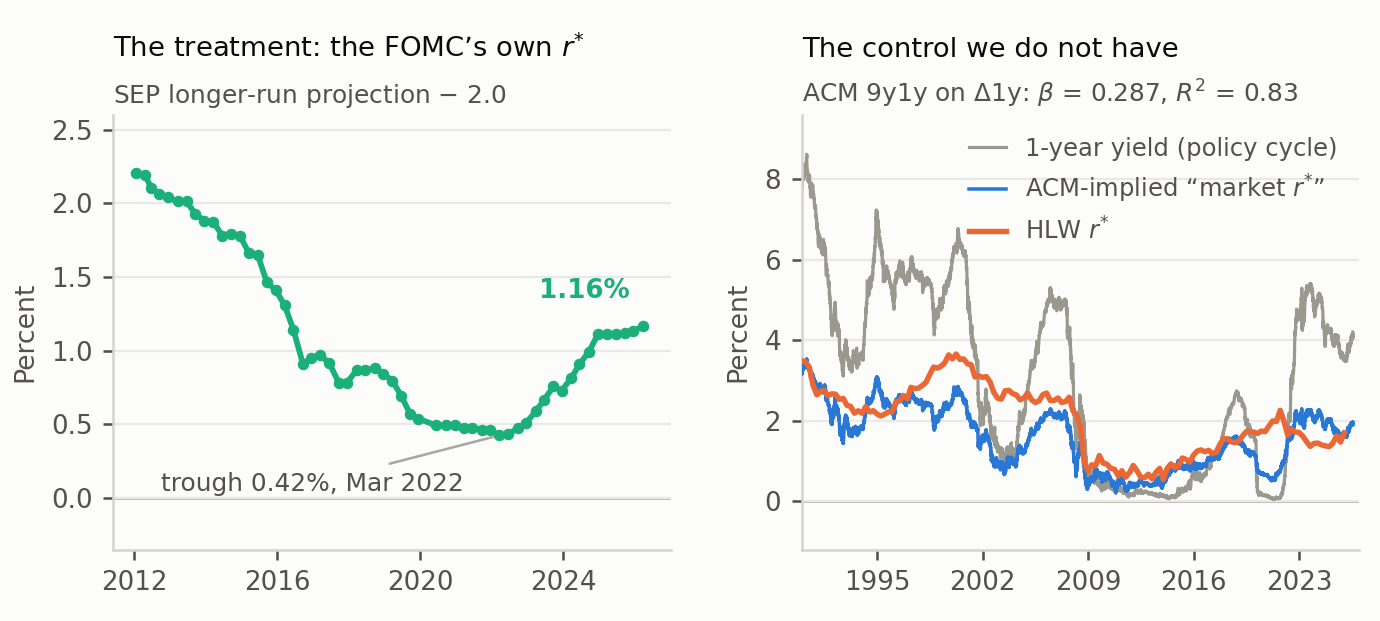
\includegraphics[width=0.95\textwidth]{s_rstar.png}
\caption{\textbf{An observable treatment and an unmeasurable control.} Left: the FOMC's own
\rs{}, the SEP longer-run projection less 2.0. Right: the ACM-implied ``market \rs{},'' the
one-year yield, and HLW \rs{} for comparison.}
\label{fig:rstar}
\end{figure}

\subsection{And the treatment window is the wrong decade}

Even setting the measurement problem aside, the design is defeated by timing. Splitting the
in-window drift by period:

\begin{center}\small
\begin{tabular}{lrrrr}
\toprule
Period & Meetings & bp/meeting & $t$ & Cumulative\\ \midrule
Jun 1989 -- Dec 2011 (pre-SEP) & 245 & $-2.46$ & $-3.06$ & $\mathbf{-5.85}$ pp\\
Jan 2012 -- Mar 2022 (dot falling 1.78 pp) & 85 & $-0.40$ & $-0.41$ & $-0.23$ pp\\
Mar 2022 -- Jul 2026 (dot rising 0.74 pp) & 35 & $-3.49$ & $-1.53$ & $-1.16$ pp\\
\bottomrule\end{tabular}
\end{center}
\vspace{-0.3em}
{\footnotesize\noindent The cumulative column sums daily in-window changes; days shared by
adjacent events are counted once.}

\vspace{0.4em}
\noindent Two things follow. First, \textbf{81\% of the in-window decline is complete before the
dot plot begins} (Figure~\ref{fig:timing}). The period in which the Fed's endpoint view is
observable is the period in which the phenomenon being explained is essentially absent.
Every projection-based test of the information channel --- including the published one --- is
run where there is little left to explain.

Second, during the decade when the FOMC cut its own longer-run rate by 1.78 pp --- the
episode in which an information channel should be loudest --- the in-window contribution is
$-0.40$ bp per meeting with $t=-0.41$. Indistinguishable from zero.

\begin{figure}[tbp]
\centering
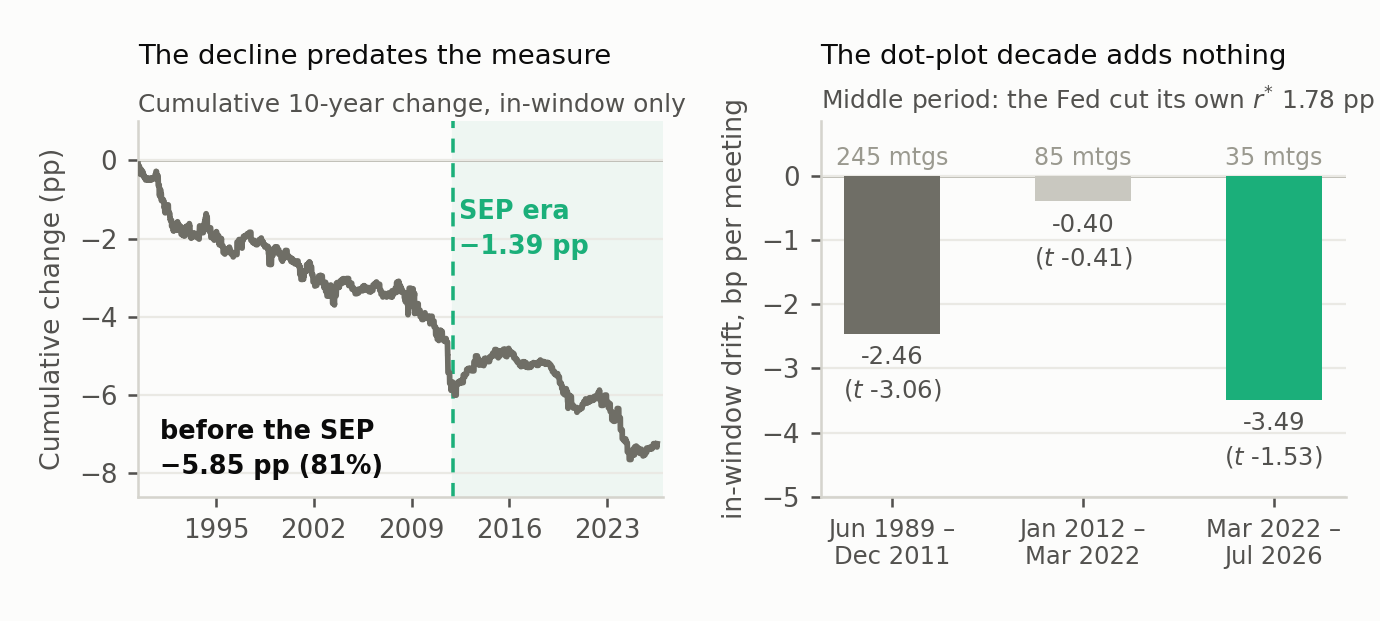
\includegraphics[width=0.95\textwidth]{s_timing.png}
\caption{\textbf{The effect and the measurement do not overlap in time.} Left: cumulative
in-window decline, with the SEP era shaded. Right: in-window drift per meeting by period.}
\label{fig:timing}
\end{figure}

% =====================================================================
\section{What survives}

\begin{center}\small
\begin{tabular}{@{}p{0.28\textwidth}p{0.36\textwidth}p{0.28\textwidth}@{}}
\toprule
\textbf{Result} & \textbf{Identifying assumption} & \textbf{Status}\\ \midrule
Event-list reconciliation: TP share 91\% $\to$ 46\% & None beyond the ACM series being the
same object in both papers & Finished; most immediately publishable\\[0.3em]
ACM is a fixed filter, $R^2=1$, $c'\mathbf 1 = 0.529$ & Spanning; ACM's own estimated loadings
& Finished; theorem standard, application new\\[0.3em]
Timing fact: 81\% pre-dates the SEP & Window assignment only & Finished; reframes the
projection-based literature\\[0.3em]
2022--26: tightening occurs entirely outside windows & Window assignment only & Finished; no
other paper covers it\\[0.3em]
Fed--market wedge design & Requires a non-circular market endpoint & \textbf{Set aside} --- no
such measure available\\
\bottomrule\end{tabular}
\end{center}

\vspace{0.3em}
\noindent Two further lines were considered and dropped. A credibility asymmetry between
dovish and hawkish signals is underpowered (18 upward revisions gives 21--31\% power), and
Hillenbrand's own Table 5 and Figure 11 already split by direction while the ratchet
mechanism is Rungcharoenkitkul, Borio \& Disyatat (BIS WP 817). Expectations versus term
premium as a standalone question is contested by the two papers above and unidentifiable for
the reason in \S4.3.

% =====================================================================
\section{The unanswered question I would build on}

Return to Figure~\ref{fig:persist}. Window and non-window days have nearly identical daily
volatility (6.72 versus 5.60 bp) but completely different cumulative outcomes ($-6.16$ versus
$-0.82$ pp). The drift-to-noise ratio is roughly 45 times higher inside the window.

So the question is not which component moves. It is:

\begin{quote}
\textbf{Why do only scheduled-date price changes persist?}
\end{quote}

A long-horizon variance-ratio decomposition estimated separately by day type converts this
from a description into a measured object: the permanent share of a day's innovation,
estimated for window days and non-window days separately, over horizons of one month to two
years. It requires no decomposition, no endpoint measure and no model of the term premium ---
so it survives every identification problem above. It also confronts Hanson--Lucca--Wright
(reversal) with Hillenbrand (permanence) directly, on a statistic that neither reports.

% =====================================================================
\section{Path forward}

\subsection*{Immediate (four weeks)}

\noindent\textbf{(a) The issuance test.} Lou, Pintér, Üslü \& Walker (BIS WP 1232) document a
supply-driven pre-announcement drift in UK gilts and claim Hillenbrand's effect concentrates
in FOMC windows \emph{without} long-dated Treasury issuance. If correct, the mechanism is
dealer inventory rather than monetary policy. Auction dates are public; this is a few days'
work and it is decisive either way.

\noindent\textbf{(b) Draft the reconciliation note} --- Extension 1 plus the timing fact in \S5.3.
Self-contained, model-free, and it resolves a live disagreement.

\subsection*{Medium term (one term)}

\noindent\textbf{(c) Permanent versus transitory by day type} --- the variance-ratio design in \S7.
This is the direction I think is most promising and the one I would build a chapter around.

\subsection*{Contingent}

\noindent\textbf{(d) Extend the Fed-side measure back before 2012}, where the effect actually
lives, using Tealbook/Greenbook projections (available 1981--2019 with the five-year lag). This
is the only way to test any projection-based mechanism on the sample that contains the
phenomenon.

% =====================================================================
\section{Where I would value guidance}

\begin{enumerate}\setlength\itemsep{0.15em}
\item Whether the reconciliation is better as a standalone short submission or folded into a
chapter as a methodological section.
\item Access to Blue Chip Financial Forecasts long-range and to the Tealbook archive --- both
are binding constraints on (d).
\item Whether the permanent/transitory framing in (c) is the right way to pose the question,
or whether it is too descriptive to carry a chapter without a mechanism.
\end{enumerate}

\vspace{0.8em}
\noindent\rule{\textwidth}{0.4pt}\\[0.3em]
\footnotesize\textbf{Data.} Gürkaynak--Sack--Wright zero-coupon yields; Adrian--Crump--Moench
daily decomposition, June 1989 -- August 2026; FOMC calendar assembled from Federal Reserve
historical meeting pages (300 scheduled meetings 1989--2026 plus 73 conference calls and
unscheduled actions); SEP dot-plot archive, 57 meetings, January 2012 -- March 2026. All
estimates recomputed from source; nothing taken from a prior write-up.

\end{document}
